\section{Introduction}

The Kochen--Specker (KS) theorem~\cite{KochenSpecker1967} shows that quantum observables cannot
be assigned definite values independently of the measurement context (for a review see
Ref.~\cite{Budroni2022}).  It is proved by exhibiting a finite set of rays in Hilbert space that
admits no $\{0,1\}$-valued assignment compatible with orthogonality.  Dimension three is the
smallest in which such sets exist.  (Smaller sets exist in higher dimensions, for example 20
vectors in dimension four~\cite{Kernaghan1994} and 36 in dimension
eight~\cite{KernaghanPeres1995}.)  In dimension three the smallest known set is the 31-ray
configuration of Conway and Kochen ($\CK$), reported by Peres~\cite{Peres1993}; the best lower
bound is 24, obtained for real vectors by Kirchweger, Peitl and
Szeider~\cite{KirchwegerPeitlSzeider2023} and for real and complex vectors by Li, Bright and
Ganesh~\cite{LiBrightGanesh2024}, improving the earlier 22 of Uijlen and
Westerbaan~\cite{UijlenWesterbaan2016}.  Trandafir and Cabello~\cite{TrandafirCabello2025} proved
that the orthogonality relations of $\CK$ have a unique realization up to unitary equivalence,
and that no set of 30 or fewer rays arises from one specified construction starting from the
Yu--Oh set; that 31 is the minimum without that assumption remains a conjecture.

\paragraph{The alphabet.}
Peres drew his two three-dimensional examples as cubes~\cite{Peres1991,Peres1993}: each ray joins
the centre of the cube to a marked point on its surface.  The two drawings differ in one respect.
In both, the marked points lie on a $5\times5$ grid on each face; for the 33-ray set the grid
lines sit at $0,\pm1,\pm\sqrt2$, and for $\CK$ at $0,\pm1,\pm2$ (Fig.~\ref{fig:triptych}).  The
list of coordinate values is thus a parameter of the construction, and one can ask what happens
when it is varied.  We call the list an \emph{alphabet} (Pavicic et
al.~\cite{Pavicic2019} speak of ``vector components''), a coordinate triple a \emph{word}, and the
set of all rays with coordinates in the alphabet its \emph{pool}.

\begin{figure}[t]
\centering
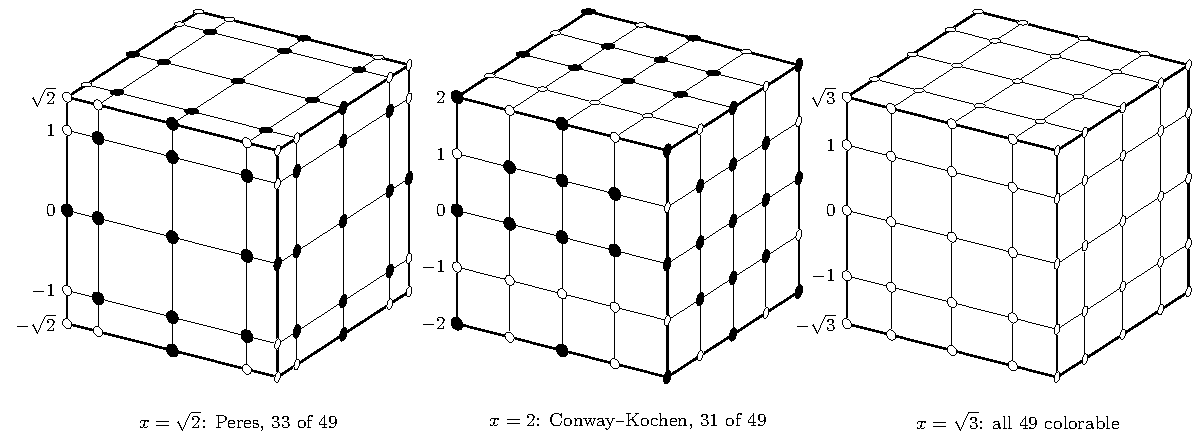
\includegraphics[width=\textwidth]{figures/alphabet_cube_triptych.pdf}
\caption{One cube, three alphabets $\{0,\pm1,\pm x\}$ with $x$ real and $x>1$.  Each of the 49
rays of the pool leaves the centre through a grid point; antipodal points are the same ray.
Filled points: the 33 rays of Peres ($x=\sqrt2$, the unique smallest uncolorable subset of that
pool) and the 31 rays of Conway and Kochen ($x=2$, one of six smallest subsets, all equivalent
under signed permutations of the axes).  At $x=\sqrt3$ the whole pool is colorable.  Only the two
inner grid lines move with~$x$.  Nearness of two points on the cube says nothing about
orthogonality of the rays, and the picture does not represent the complex pools of
Section~\ref{sec:circle}.}
\label{fig:triptych}
\end{figure}

\begin{figure}[t]
\centering
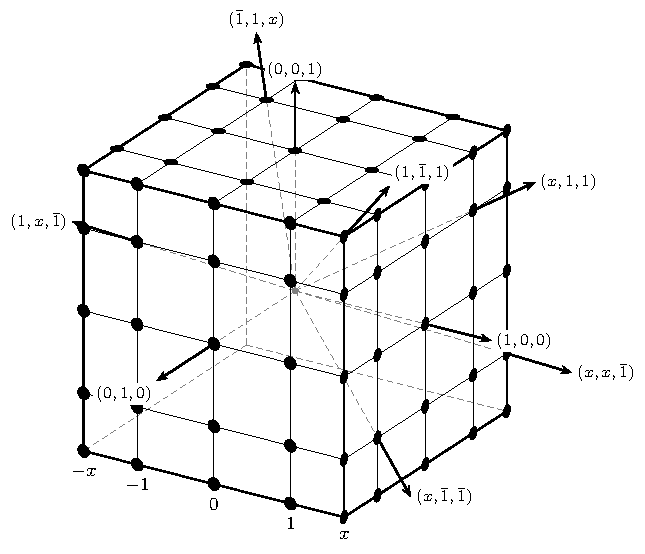
\includegraphics[width=0.6\textwidth]{figures/alphabet_cube_generic.pdf}
\caption{Words as rays.  A ray whose coordinates form a word over $\{0,\pm1,\pm x\}$ leaves the
centre of the cube $[-x,x]^3$ through a grid point; a bar is a minus sign.  Words without the
letter~$x$, such as $(1,0,0)$ and $(1,\bar1,1)$, reach the surface after scaling by~$x$.  The
49 rays are the same list of words for every~$x$; which pairs are orthogonal is not.  For
example $(x,1,1)\cdot(x,\bar1,\bar1)=x^2-1-1$, which vanishes only for $x^2=2$.}
\label{fig:generic}
\end{figure}

\paragraph{Results.}
For a family of alphabets depending on parameters, the question is which parameter values give
an uncolorable pool and how small a KS set the pool then contains.  For three families we
classify colorability completely and determine every minimum except at two classes of points of
the third family.

\begin{enumerate}[label=(\roman*)]
\item \emph{Two-symbol alphabets $\{0,\pm1,\pm x\}$, $x$ complex} (Theorem~\ref{thm:twosymbol}).
The pool is uncolorable only at isolated points: $x$ or $1/x$ one of $\pm2$, $\pm\sqrt2$,
$\pm\sqrt{-2}$, or $x$ a primitive third or sixth root of unity.  No KS set with coordinates in
a two-symbol alphabet has fewer than 31 rays.
\item \emph{Real three-symbol alphabets $\{0,\pm1,\pm x,\pm y\}$} (Theorem~\ref{thm:threesymbol}).
After normalization to $1<x<y$, the pool is uncolorable on six curves, where two letters have
ratio 2 or~$\sqrt2$, and at eight further points.  Again no KS set has fewer than 31 rays.
\item \emph{Conjugate-closed alphabets $\{0,\pm1,\pm x,\pm x^{*}\}$, $x$ complex}
(Theorem~\ref{thm:conj}, Fig.~\ref{fig:circle}).  The pool is uncolorable exactly on two
circles, four lines through the origin with the origin removed, and four further points.  On
the circle $|x|^2=2$ one fixed list of 45 words is uncolorable at every point and no shorter
fixed list is
(Theorem~\ref{thm:circle}); the circle $|x|^2=\tfrac12$ carries the 33-ray family of Gould and
Aravind.
\end{enumerate}

A fourth family has a discrete parameter: the pool of $0$ and the $n$th roots of unity is
uncolorable exactly when $6\mid n$ (Theorem~\ref{thm:6n}).  Section~\ref{sec:catalogue} adds
pools that lie outside these families, each with exact counts and either a certified minimum or
a stated upper bound.

\paragraph{Standard of proof.}
Each of the three continuous-parameter classifications reduces, by an argument given in the
text, to finitely many cases that are decided in exact arithmetic by named scripts.  The
roots-of-unity theorem has a structural proof for every~$n$, with one finite computation at
$n=6$.  In addition the following are proved in the Lean
proof assistant and checked by its kernel (Section~\ref{sec:methods}): Theorem~\ref{thm:6n} for
$n\ge3$; the uncolorability of the 45 words for every $x$ on the circle; and the minimum KS
subsets of six pools (31, 33, 33, 33, 43 and 47 rays).

\paragraph{Relation to earlier versions.}
Versions 1--9 of this paper proposed a classification by ``cancellation mechanisms'' and
described the uncolorable alphabets as isolated ``islands''.  That proposal did not survive
checking and was withdrawn in version~10; Appendix~\ref{sec:corrections} lists the withdrawn
claims.  The present version restates the results that replaced it.  Since the uncolorable
alphabets are not isolated, we do not use the word ``island''.

\section{Definitions and methods}\label{sec:prelim}

\begin{definition}
A \emph{ray} in $\C^3$ is a one-dimensional subspace, written $[v]$ for a nonzero vector~$v$.
Rays $[v],[w]$ are \emph{orthogonal} if $\braket vw=\sum_k v_k^{*}w_k=0$.  A \emph{triad} (or
\emph{basis}) is a set of three mutually orthogonal rays.
\end{definition}

\begin{definition}
A \emph{coloring} of a set $S$ of rays is a map $f:S\to\{0,1\}$ such that (a)~no two orthogonal
rays of $S$ both receive~1, and (b)~every triad contained in $S$ has exactly one ray with value~1.
$S$ is \emph{KS-uncolorable}, or a \emph{KS set}, if it has no coloring.  Its \emph{orthogonality
graph} has the rays as vertices and the orthogonal pairs as edges; the triads are its triangles.
Both the edges and the triangles enter the definition, and an edge lying in no triangle of $S$
is still a constraint.
\end{definition}

A coloring of $S$ restricts to a coloring of any subset, because every orthogonal pair and every
triad of the subset is one of~$S$:

\begin{lemma}[Restriction]\label{lem:restrict}
A set of rays that contains an uncolorable subset is uncolorable.
\end{lemma}

\begin{definition}
An \emph{alphabet} is a finite set $\mathcal A\subset\C$ containing~0.  Its \emph{raw pool} is
\[
S(\mathcal A)=\{\,[v]: v\in\mathcal A^3\setminus\{0\}\,\}.
\]
The \emph{completed pool} $\bar S(\mathcal A)$ is the smallest set of rays containing
$S(\mathcal A)$ and containing, with every orthogonal pair $[v],[w]$, the third ray of their
triad, $[(v\times w)^{*}]$ (the ordinary cross product for real vectors).  In all cases reported
here the completion was computed to closure and is finite; we do not know a general finiteness
criterion.
\end{definition}

In a completed pool every orthogonal pair lies in exactly one triad, so the numbers of pairs $E$
and triads $T$ satisfy $E=3T$.  This is a convenient check: the raw Eisenstein pool has
$E=174$, $T=22$, so it is not closed, contrary to a statement in version~9.

\paragraph{Three cautions on scope.}
(1)~Uncolorability is a property of a pool, not of a ring or a field.  Every ring that appears in
this paper contains $\Z$ and therefore contains the coordinates of $\CK$; the statement ``this
field supports a KS set'' is true of all of them and distinguishes nothing.  (2)~The size of a
generator is not an invariant of the pool: multiplying every word by $x^{-1}$ shows
$S(\{0,\pm1,\pm x\})=S(\{0,\pm1,\pm x^{-1}\})$, and $S$ is also unchanged by $x\mapsto-x$.
(3)~A raw pool and its completion are different objects.  Their counts and minima need not
agree; inclusion gives only one-way implications (if the raw pool is uncolorable so is its
completion, and a KS subset of the raw pool bounds the minimum of the completion from above).
Every count below says which pool is meant.

\subsection{Methods}\label{sec:methods}

\paragraph{Exact arithmetic.}  Coordinates are elements of a number field $\Q[t]/(m(t))$ stored
as rational coefficient vectors; rays are compared after division by the first nonzero
coordinate; a pair is orthogonal when the Hermitian product is the zero element.  The
cyclotomic pools use exponents modulo~$n$, and the proof of Theorem~\ref{thm:circle} uses
integer polynomial identities.  No count in Sections~\ref{sec:real}--\ref{sec:catalogue} depends
on a floating-point tolerance.  The only floating-point quantities in the paper are the flex
counts of Section~\ref{sec:rigidity}; they are labelled as numerical.  Floating-point
evaluation is used elsewhere only as a cross-check of exact computations.

\paragraph{Colorability.}  Colorability of a finite set is decided by a SAT
solver~\cite{AudemardSimon2018}: one variable per ray, a clause forbidding two 1s on each
orthogonal pair, and a clause requiring at least one 1 on each triad.

\paragraph{Certified minima.}  Let $P$ be an uncolorable pool.  If $M\subseteq P$ is colorable
then, by Lemma~\ref{lem:restrict}, every uncolorable subset of $P$ contains a ray outside~$M$.
The certifier keeps a list of such sets $M$, each verified colorable by the SAT solver, and asks
a second solver for a set $R$ of fewer than $u$ rays meeting the complement of every listed~$M$,
where $u$ is the size of the best uncolorable subset found so far.  If $R$ is uncolorable, $u$
decreases; if $R$ is colorable it is enlarged to a colorable set $M\supseteq R$ and $M$ joins the
list.  When no such $R$ exists, no uncolorable subset has fewer than $u$ rays, and the minimum is
exactly~$u$.  The answer is correct whenever the SAT solver is.  The list of sets $M$ is in principle a
certificate that can be checked independently.  For six pools it is checked in Lean (below);
for Theorem~\ref{thm:circle} it is archived; the other minima are reproducible by re-running
the scripts.  Minima that the procedure did not finish within
its time budget are reported as upper bounds.

Two reductions speed up the runs for Theorems~\ref{thm:conj} and~\ref{thm:threesymbol}; both
keep the answer exact.  First, if a ray of an uncolorable set lies in no triad of that set,
deleting it leaves an uncolorable set (a coloring of the rest extends by giving the ray~0).  So a
minimum set lies in the \emph{core} of the pool, obtained by deleting rays that lie in no triad
until none is left, and the search is run there.  Second, if
$g$ is a permutation of the rays preserving orthogonality and $M$ is colorable, so is $g(M)$, so
each colorable $M$ may be added to the list together with all its images under a group of such
permutations (signed permutations of the coordinates, and complex conjugation where the alphabet
is closed under it; each is checked to preserve the graph before use).

The same enumeration, continued after the first
minimum set is found, lists \emph{all} minimum sets of a pool.

\paragraph{Proofs checked in Lean.}  Three files in the repository are checked by the kernel of
Lean~4 (with the mathlib library) and use no axioms beyond the standard three.  Where a proof
rests on a finite set of rays, their coordinates are exact elements of a ring written as
integer tuples, orthogonality is recomputed inside Lean, and the certificates, which are
computed outside Lean, are checked there and not trusted.
\texttt{Cyclotomic6n.lean} proves Theorem~\ref{thm:6n} for $n\ge3$.
\texttt{NamedSets.lean} proves that the 43-ray set, the 47-ray set and, for every $x$ with
$|x|^2=2$, the 45 words of Theorem~\ref{thm:circle} are uncolorable, each from a case-split
refutation.  \texttt{Minimality.lean} proves minima.  Its certificate for a pool with minimum
$u$ is the list of colorable sets $M$ described above, each with a coloring, together with a
branching proof that no set of fewer than $u$ rays meets the complement of every~$M$: a node
puts one ray in or out, and a leaf names complements that avoid the rays put in and are pairwise
disjoint once the rays put out are removed, so that a set meeting all of them needs a separate
ray for each.  A soundness theorem for this checker is proved once.  The result for each of six
pools, those of $\{0,\pm1,\pm2\}$, $\{0,\pm1,\pm\sqrt2\}$, $\{0,\pm1,\pm\sqrt{-2}\}$, the
Eisenstein alphabet, $\{0,\pm1,\pm\alpha,\pm\alpha^{*}\}$ with $\alpha=(1+\sqrt{-7})/2$, and
$\{0,\pm1,\pm\psi,\pm\psi^2\}$ with $\psi^3=\psi^2+1$, is a theorem with two halves: some $u$ of
the pool's vectors form an uncolorable set, and every set of fewer than $u$ of them has a
coloring.  Three limits should be stated.  First, in Lean each pool is an explicit list of
vectors; that the list consists of all rays with coordinates in the alphabet is not proved
there.  Second, the Lean statements are about sets of vectors, not rays.  This loses nothing,
by an argument that is not itself formalized: a coloring of rays gives a coloring of any choice
of representative vectors and conversely, and each listed pool has one vector per ray (the
export script checks this), so the minimum for vectors is the minimum for rays.  Third, these are minima within a pool; they
say nothing about KS sets outside it.

The procedure used in earlier versions (described there as ``OCUS'') was different and was not
sound: when a candidate was colorable, it required the next candidate to contain a ray that
completes a violated triad with \emph{two} rays of the current candidate, ignoring triads with
two or three rays outside it.  That can exclude genuine uncolorable subsets, and it did: it
reported 52 for the completed golden-ratio pool, which contains an uncolorable subset of~51.
None of the minima in this version comes from that code.
